\section{Conditioning and reference matching resolve diversity reversals}
\label{sec:supp_t2i}

\subsection{Independent prompts, random streams, and evaluation units}
We use the complete public PartiPrompts~\cite{yu2022parti} prompt list, retaining its category and
challenge annotations. A fixed permutation (NumPy seed 20261015) selects 32
representation-fit prompts, 48 development prompts, 128 evaluation prompts, and
256 separate calibration prompts. Selection precedes generation and does not
inspect prompt wording or image outcomes. All 464 selected rows have unique
identifiers and unique casefolded, whitespace-normalized prompt strings, with
no exact text duplicate across splits. The reference fit pool contains 16
images per prompt; calibration uses one independently seeded image per prompt.
Development uses eight images per prompt. Evaluation uses eight diagnosis seeds
and 16 separate outcome seeds per prompt. All arm-level headline results use
only the 16 outcome seeds, giving 2,048 images per arm and 128 independent prompt
units. The eight diagnosis images implement a frozen action-selection rule;
they never enter the outcome estimate.

The initial seed is the split-specific offset plus 1,000 times the original
PartiPrompts row index plus the replicate index. Noise is drawn in CPU FP32 and
then converted to the model's native precision. Every method within a family
receives the same initial noise. Separate random streams, offset by $10^8$,
$2\!\times\!10^8$, and $3\!\times\!10^8$, supply stochastic scheduler updates,
conditional CADS perturbations, and unconditional CADS perturbations. The
Stable Diffusion evaluation offset is $10^7$; Sana uses $2\!\times\!10^7$.
The fit, calibration, development, and reference-refinement streams are disjoint
from evaluation. Saved configuration files list every prompt and seed; a
collision audit checks the generated initial-noise streams.

Let $p$ index the $N_{\rm p}$ evaluation prompts, and let $X$ and
$X_{\rm ref}$ denote candidate and reference images at that prompt.
For a representation $\phi$, the primary conditional spread ratio
uses sample covariances within prompts:
\begin{equation}
 R_\phi=\frac{N_{\rm p}^{-1}\sum_{p=1}^{N_{\rm p}}\operatorname{tr}
 \widehat{\operatorname{Cov}}(\phi(X)\mid p)}
 {N_{\rm p}^{-1}\sum_{p=1}^{N_{\rm p}}\operatorname{tr}
 \widehat{\operatorname{Cov}}(\phi(X_{\rm ref})\mid p)}.
\label{eq:supp_prompt_spread}
\end{equation}
Each prompt is centered separately and receives equal weight. This differs from
both a pooled covariance, which includes differences between prompts, and the
mean of promptwise variance ratios. We retain these alternatives as sensitivity
analyses. Intervals resample paired prompt units, preserving all seeds and all
methods within each sampled prompt. Arm and representation intervals are
descriptive 95\% intervals; the frozen policy's four primary contrasts use
98.75\% intervals. Fixed-prompt occupancy inference is kept separate from this
population-over-prompts analysis.
The saved representation analysis additionally retains an approximate simultaneous
95\% max-standardized-log-ratio bootstrap check across its 20 fixed contrasts.
A directional interval excluding 1 does not by itself pass the operational
0.9/1.1 contraction/expansion margins or the accompanying quality/support gates.

To explain a pooled/conditional reversal, we retain the exact balanced-design
ANOVA decomposition. With $N_{\rm p}$ prompts and $m$ samples per prompt,
let $W$ be the mean within-prompt sample covariance trace and $B_{\rm obs}$
the sample covariance trace of prompt means. The sample covariance trace
$T_{\rm pooled}$ across all images is
\begin{equation}
 T_{\rm pooled}=\frac{N_{\rm p}(m-1)}{N_{\rm p}m-1}W
              +\frac{m(N_{\rm p}-1)}{N_{\rm p}m-1}B_{\rm obs}.
\label{eq:supp_prompt_anova}
\end{equation}
We verify this identity numerically for every arm and representation. The
classical correction $B_{\rm obs}-W/m$ removes estimated finite-seed noise
from the prompt-mean covariance under independent seed draws; negative
estimates are retained. This is a descriptive variance-component analysis,
not a new estimator or a decision gate. The extension that retains both additive terms and this correction was
specified after access to the DDIM4 outcome contrast. It covers all 29 SD
and seven Sana arms using the same 128 prompts and 16 outcome seeds. The complete tables normalize both contributions by the common reference's
pooled trace and retain paired prompt-bootstrap intervals for between-prompt
ratios. For DINO, reference within/between contributions 0.400/0.600 become
0.523/0.396 under DDIM4. Their sum is the pooled ratio 0.919; dividing
within-prompt variation by the reference within component gives 1.306.
This secondary descriptive decomposition explains the reversal without
changing any primary comparison or gate.

\subsection{Native model configurations}
\paragraph{Stable Diffusion.}
All images are $512\!\times\!512$ pixels. The base model is SD1.5
\cite{rombach2022ldm}; DINOv2-base \cite{oquab2024dinov2} and CLIP ViT-L/14-336
\cite{radford2021clip} provide independent image representations. DINO uses the
raw 768-dimensional final class token; CLIP uses its normalized 768-dimensional
image embedding. CLIP prompt--image cosine similarity is computed with the
same frozen encoder. All 464 selected prompts fit both tokenizers: the maximum
is 63 tokens, including start/end tokens, below the 77-token limit.
The reference sampler is 50-step leading-schedule DDIM, with guidance 7.5 as the
common comparison. Additional reference pools at guidance 1.75 and 1 support
explicitly identified reference-sensitivity analyses.

\paragraph{Native distillation.}
LCM-LoRA \cite{luo2023lcmlora} uses its native LCMScheduler at four or eight
steps, with external guidance disabled. Its external guidance value of 1 does
not identify the effective guidance embedded during distillation; comparison
with a CFG-1 base reference is therefore a numerical-guidance sensitivity.
The official adapter card does not identify a unique fixed training guidance;
the official LCM-LoRA training example samples a range of teacher guidance
values while validating with external guidance 1. DMD2
\cite{yin2024dmd2} uses the released SD1.5
\texttt{fid8.35\_checkpoint\_model\_041000} checkpoint. In the native
recipe, $z$ is the starting noise latent, $c$ the prompt conditioning,
$\epsilon_\theta$ the noise predictor with frozen checkpoint parameters $\theta$,
and $z_0$ the clean
latent estimate. The decoder $\operatorname{Dec}$ maps the rescaled
latent to image $x$. The single prediction at timestep 999 uses
cumulative signal coefficient 0.0047 and latent scale 0.18215:
\begin{equation}
 \begin{aligned}
 z_0&=\frac{z-\sqrt{1-0.0047}\,\epsilon_\theta(z,999,c)}{\sqrt{0.0047}},\\
 x&=\operatorname{Dec}(z_0/0.18215).
 \end{aligned}
\label{eq:supp_dmd2_step}
\end{equation}
We strictly load every checkpoint tensor and use freshly loaded FP32 text
encoder, denoiser, and VAE weights, with TF32 enabled as in the official
implementation. The matched teacher guidance is 1.75;
common-reference guidance 7.5 and guidance 1 are also reported. A multi-step
LCM schedule is not an eligible implementation of this DMD2 checkpoint.

\paragraph{Learned flow.}
Sana-600M \cite{xie2025sana} is evaluated at its native 512-pixel resolution,
with a Gemma text encoder, deep-compression autoencoder, and guidance 5. The
pinned public checkpoint is
\texttt{Sana\_600M\_512px\_diffusers}, revision
\texttt{83d7a190bfd1fd070570\allowbreak{}a793d2dab5c7a3231b9d}. Its native Flow-DPM++
configuration uses flow prediction, second-order midpoint updates, flow-shift
3, and a zero terminal sigma. We compare its 50-step reference, native
20-step setting, four/eight-step Flow-DPM++, four/eight-step shifted Euler, and
eight-step CADS--Flow-DPM++. Euler uses its native shifted time grid; this is a
comparison of practical solver configurations, not an isolated change in order.
The transformer uses FP16 and the text encoder and autoencoder use BF16, as in
the public recipe. We retain the native complex-instruction prefix and
300-token text-encoder limit; the exact instruction is saved with the run.
Independent Sana reference samples fit and calibrate its
support scores; SD feature thresholds are not reused across model families.
The numerical decision margins and routing rule transfer without retuning.

\subsection{Interventions and closest comparisons}
\begin{table*}[t]
\centering\small
\begin{tabular}{llll}
\toprule
SD1.5 comparison & Sequential denoiser calls & Guidance & Configuration \\
\midrule
DDIM reference & 50 & 7.5, 1.75, 1 & Leading schedule \\
DDIM & 4, 8 & 7.5 & Leading schedule, deterministic \\
DDIM trailing & 4, 8, 16 & 7.5 & Trailing schedule \\
Stochastic DDIM & 4, 8 & 7.5 & $\eta=1$ \\
Reduced guidance & 4, 8 & 3 & Leading DDIM \\
DPM++ / UniPC & 4, 8, 16 & 7.5 & Order 2, linspace schedule \\
CADS--DDIM & 4, 8 & 7.5 & Published annealing parameters \\
CADS--DPM++ & 4, 8, 16 & 7.5 & Published annealing parameters \\
Tuned CADS--DPM++ & 8 & 7.5 & Secondary frozen development choice \\
LCM-LoRA & 4, 8 & External 1 & Native LCM scheduler \\
Hybrid LCM-LoRA & 4, 8 & First 5; then external 1 & First step uses base denoiser \\
DMD2 & 1 & Distilled 1.75 & Native epsilon-to-$z_0$ conversion \\
\bottomrule
\end{tabular}
\caption{Complete SD evaluation: 28 primary arms, including three named
references, and one separately frozen tuned-CADS arm. Guided base samplers use
two denoiser example evaluations per sequential call. Native LCM uses one;
hybrid LCM uses five/nine examples for four/eight calls; DMD2 uses one.}
\label{tab:t2i_arms}
\end{table*}

CADS \cite{sadat2024cads} follows the original equations and algorithm: every
step perturbs the original text embedding, with independent noise on both CFG
branches, then restores its mean and standard deviation. Published SD
annealing parameters are $(\tau_1,\tau_2,s,\psi)=(0.6,0.9,0.25,1)$.
We hold guidance at 7.5 for controlled SD comparisons; this is not a reproduction
of the paper's longer-schedule, guidance-9 headline experiment. A compact
development sweep evaluates $(s,\tau_1,\tau_2)=(0.1,0.6,0.9)$,
$(0.1,0.8,1)$, and $(0.25,0.8,1)$ alongside the published setting, using the
first 16 development prompts and their eight paired seeds. All four settings
are retained. The strongest development preference, $s=0.1$ and
$(\tau_1,\tau_2)=(0.8,1)$, is frozen as a secondary held-out comparison;
it does not change the primary policy. Full sweep results are included below.
For Sana, CADS applies the same published perturbation parameters to the native
conditioning embeddings while preserving the original attention masks; this
flow-family adaptation receives no additional parameter tuning.

The hybrid LCM comparison adapts the official first-base-step procedure of
Gandikota and Bau \cite{gandikota2026diversity} from SDXL to SD1.5 LCM-LoRA.
It preserves the LCM timestep sequence, uses the base denoiser at the first
step with the official CLI guidance of 5, and then uses LCM with external
guidance disabled. We explicitly identify this model-family adaptation.
The additional base step's CFG branch is counted in computational cost.
This hybrid has no single guidance-matched teacher; its primary comparison uses
the common CFG-7.5 reference.

\subsection{Quality, support, and competing diversity measures}
PickScore \cite{kirstain2023pickapic} supplies a frozen human-preference
\emph{proxy}, distinct from the generator and the DINO/CLIP audit encoders.
Let $s$ index $N_{\rm s}$ seeds per prompt and let $X_{p,s},X^{\rm ref}_{p,s}$
be the matched candidate and reference images. The quality statistic is
\begin{equation}
 \begin{aligned}
 \psi&=\frac{1}{N_{\rm p}}\sum_p\frac{1}{N_{\rm s}}\sum_s
 \operatorname{sigmoid}(\Delta\ell_{p,s}),\\
 \Delta\ell_{p,s}&=\ell(X_{p,s},p)-\ell(X^{\rm ref}_{p,s},p),
 \end{aligned}
\label{eq:supp_pickscore_preference}
\end{equation}
where $\ell$ is the model's scaled cosine logit. This averages probabilities
directly; sigmoid of an averaged logit difference is a different statistic.
A preference floor of 0.45 allows five percentage points below model
indifference. The lower confidence bound must meet that floor for a quality
pass; an interval spanning the threshold remains unresolved. This is not a
human-study equivalence claim. CLIP alignment has a separately fixed loss
tolerance of 0.01. Sensitivities use preference floors 0.475/0.45/0.40,
alignment tolerances 0.005/0.01/0.02, support-tail excess margins
0.025/0.05/0.10, and spread retention 0.95/0.90/0.80.

Each image representation fits a 32-dimensional reference PCA, ten support
regions, and a nearest-reference support score using the fit pool only.
The independent 256-prompt calibration pool determines the 95th-percentile
support threshold. The population outcome analysis averages support-tail
excess within prompts and bootstraps prompt units. Fixed-prompt regional mass
bounds instead use simultaneous exact binomial bounds, with a declared family
over regions, prompts, representations, arms, and references. Sixteen images
per prompt generally cannot resolve rare regional probability loss; an
inconclusive occupancy test is never evidence that deletion is absent.
PartiPrompts contains prompts, not a paired image population, so support and
coverage here are relative to the named generator reference.

\paragraph{Native reference gates.}
Against the common CFG-7.5 reference, LCM4, LCM8, and DMD2 pass both feature
support gates but fail the preference floor. DMD2 against its matched CFG-1.75
teacher passes support and reaches preference 0.558, while its DINO/CLIP spread
ratios of 0.901/0.907 remain unresolved at the 0.9 contraction margin.
Against the CFG-1 sensitivity reference, LCM4/8 improve preference to
0.731/0.712 but fail CLIP support compatibility: their support-tail excess
intervals are [0.143, 0.226]/[0.165, 0.249], exceeding the 0.05 margin.
DINO support passes in both cases. These reference-compatibility failures
coexist with improved preference; we report spread directions without a joint
contraction assignment. All intervals in this paragraph are descriptive
95\% paired prompt-bootstrap intervals.

Scendi \cite{ospanov2025scendi} measures prompt-aware diversity through the
Schur complement of CLIP embeddings. Together with Conditional Vendi, it
addresses the important distinction between prompt variation and image
variation. The audit builds on this established distinction by jointly specifying a
named reference, an effect-size resolution, quality/support requirements,
and an independently evaluated intervention comparison.

Conventional PRDC \cite{naeem2020density} uses Euclidean DINO distances with
$k=3$ neighbors within each prompt. We report both within-prompt Vendi
\cite{friedman2023vendi} and the distinct Conditional Vendi/Conditional RKE
definitions of Jalali et al.\ \cite{jalali2026conditional}, using image/text
cosine Gram matrices and their Hadamard product. The latter are computed on
the complete outcome subset and match the official implementation numerically.
For a single fixed prompt its text kernel is rank one, so Conditional Vendi
reduces to ordinary within-prompt Vendi; this is the quantity available to a
promptwise routing baseline. Averaging such scores is not the global
cross-prompt Conditional Vendi statistic.
Delete-one-prompt sensitivity and jackknife standard errors describe their
stability. We do not report naive row-bootstrap intervals for these nonlinear
Gram statistics: duplicated prompt blocks alter their finite-sample entropy.

\subsection{Reference refinement and numerical validation}
Before evaluation, the first 16 shuffled development prompts receive eight
paired images from DDIM100 at each reference guidance and from DPM++50 at
guidance 7.5. Relative to DDIM50, DDIM100 gives conditional DINO ratios
0.962 [0.897, 1.014], 1.006 [0.994, 1.018], and 1.006 [0.992, 1.018] at
guidance 7.5, 1.75, and 1, respectively. The paired preference at guidance
7.5 is 0.500 [0.490, 0.509]. Full sampling-latent spread increases by about
6\%, so these checks support semantic-reference stability without asserting
that every latent statistic has converged. The main representation/reference
reversals persist against the refined references. Sana has an independently
seeded 50-versus-100-step check on the same fixed 16 development prompts:
its conditional ratios are 1.006 [0.998, 1.020] in DINO,
1.024 [0.999, 1.046] in CLIP, 1.0008 [0.9984, 1.0036] in complete sampling
latents, and 1.0005 [0.9981, 1.0034] after image re-encoding. The alignment
change is $-0.00015$ [$-0.00068$, $0.00031$].
Its paired preference is 0.4953 [0.4919, 0.4985], a small shift favoring
50 steps that remains within the predeclared practical quality tolerance.

Our manual DDIM, stochastic DDIM, DPM++, UniPC, and LCM samplers match stock
diffusers within one saved 8-bit pixel quantization unit. The DMD2 conversion
matches the official formula exactly. Disabling the complete CADS perturbation
gives exact identity; moment restoration has maximum mean error
$6.1\!\times\!10^{-9}$ and zero standard-deviation error in FP32.
Setting only its noise scale to zero is not generally an identity when the
annealing coefficient is zero. Manual Sana DPM and Euler four-step latent
outputs match their native pipelines exactly. On a fixed 16-sample numerical
check, Conditional Vendi and RKE match the archived official source within
$6.3\!\times\!10^{-15}$.

A paired DMD2 precision audit compares freshly loaded FP32 auxiliary weights
with the preserved exploratory implementation that had cast FP16-rounded
weights back to FP32. Conditional DINO and CLIP ratios between these versions
are 1.0001 [0.9994, 1.0007] and 0.9994 [0.9977, 1.0010]. Final evaluation
nevertheless uses the exact original FP32 recipe. Checkpoints are pinned;
strict loading, tensor compatibility, source hashes, scheduler configurations,
and environment versions are retained with each run. A separate 64-image
development check applies the same VAE weights in FP16 and FP32 to identical
saved reference and DMD2 images: the DMD2/reference re-encoded spread ratio
changes by only 0.00245\%, demonstrating insensitivity to this precision
change in the paired development check.

\subsection{Representations, artifacts, and cost accounting}
We save all 16,384 final SD latent coordinates and all 8,192 final Sana latent
coordinates. Re-encoding the decoded 8-bit image supplies a complementary
representation: the SD VAE posterior mode, or the deterministic Sana
autoencoder output, multiplied by the model's scaling factor. This comparison
separates the sampled latent state from the state reconstructed from the
visible image. Lower-dimensional pooled latent summaries and adjacent-pixel
gradient energy are retained as descriptive checks. Per-image spatial
standard-deviation trajectories are not treated as cross-seed covariance
trajectories or as evidence for a Gaussian covariance theorem.

Lossless WebP files preserve the exact images used for feature extraction.
Every batch records prompt IDs, seeds, replicate IDs, image paths, features,
alignment, latent representations, and generation/feature/re-encoding times.
The experiment manifest checks completed sample counts, unique keys, seed
matching, and all image paths. Generation uses at most eight CPU threads per
process. SD initially runs on one H200; Sana runs concurrently on a shared H200 with an
11-GiB PyTorch allocation cap, leaving room for CUDA context memory.
Four-image autoencoder chunks keep the 16-image Sana denoiser batch below the
memory budget. Shared-GPU timings are descriptive; controlled inference cost
uses sequential denoiser calls and effective CFG branch evaluations.
Parallel SD jobs use disjoint output directories; additional workers use atomic
batch commits and guards against overlapping writers. Jobs on the shared H200 have an
18-GiB allocation cap. Concurrent-job
parity is exact on 64 development images; cross-H200 parity is exact for latents,
pixels, features, alignment, and re-encodings on 128 additional development
images spanning four configurations. Batch size, model settings, seed streams,
and sampling source are fixed. Controlled timing runs on GPU0 after its other
jobs finish, with background activity on the other H200 recorded. It recomputes
prompt encodings for both families and reports text, decoding, feature
extraction, and preference scoring separately.

Audit overhead includes all diagnosis calls, feature extraction, and support
scoring. Online search costs replay the frozen access rule on the complete
offline matrix. Fixed samplers have no online diagnostic cost. Fit and
calibration costs are reported separately. The SD display uses the three
smallest held-out prompt IDs and first four outcome seeds. Sana uses the
first four shuffled prompts and their first outcome seed. All indices
are fixed without image ranking or replacement.

\begin{table*}[t]
\centering\footnotesize
\setlength{\tabcolsep}{3.5pt}
\begin{tabular}{lrrrrr}
\toprule
Method & Calls & \shortstack{DINO spread\\ratio} & \shortstack{CLIP spread\\ratio} & \shortstack{Learned preference\\$\psi$} & \shortstack{CLIP alignment\\$\Delta$} \\
\midrule
DDIM50 (CFG7.5) & 50 & 1.00 [1.00, 1.00] & 1.00 [1.00, 1.00] & 0.500 [0.500, 0.500] & 0.000 [0.000, 0.000] \\
DDIM4 & 4 & 1.31 [1.24, 1.38] & 1.16 [1.09, 1.25] & 0.247 [0.227, 0.268] & -0.031 [-0.035, -0.026] \\
DDIM8 & 8 & 1.08 [1.05, 1.12] & 1.09 [1.05, 1.14] & 0.417 [0.403, 0.430] & -0.005 [-0.007, -0.003] \\
Trailing DDIM4 & 4 & 1.13 [1.10, 1.17] & 1.05 [1.00, 1.10] & 0.330 [0.314, 0.347] & -0.011 [-0.015, -0.008] \\
Trailing DDIM8 & 8 & 1.01 [0.99, 1.03] & 1.01 [0.99, 1.04] & 0.452 [0.443, 0.460] & -0.001 [-0.003, 0.000] \\
Stochastic DDIM4 & 4 & 1.37 [1.30, 1.45] & 1.12 [1.04, 1.20] & 0.205 [0.186, 0.224] & -0.038 [-0.043, -0.033] \\
Stochastic DDIM8 & 8 & 1.07 [1.03, 1.10] & 1.07 [1.03, 1.12] & 0.392 [0.378, 0.406] & -0.005 [-0.008, -0.003] \\
CFG3 DDIM4 & 4 & 1.34 [1.26, 1.42] & 1.10 [1.03, 1.18] & 0.197 [0.178, 0.216] & -0.050 [-0.056, -0.045] \\
CFG3 DDIM8 & 8 & 1.27 [1.21, 1.32] & 1.21 [1.15, 1.28] & 0.331 [0.314, 0.348] & -0.021 [-0.024, -0.018] \\
DPM++4 & 4 & 1.13 [1.10, 1.17] & 1.07 [1.03, 1.12] & 0.326 [0.309, 0.343] & -0.012 [-0.015, -0.009] \\
DPM++8 & 8 & 1.01 [1.00, 1.03] & 1.03 [1.01, 1.05] & 0.448 [0.440, 0.456] & -0.002 [-0.003, -0.001] \\
UniPC4 & 4 & 1.15 [1.11, 1.19] & 1.07 [1.03, 1.12] & 0.321 [0.303, 0.338] & -0.013 [-0.016, -0.010] \\
UniPC8 & 8 & 1.03 [1.01, 1.04] & 1.04 [1.02, 1.06] & 0.440 [0.432, 0.448] & -0.002 [-0.003, -0.001] \\
CADS--DDIM4 & 4 & 1.38 [1.31, 1.46] & 1.22 [1.14, 1.31] & 0.229 [0.209, 0.249] & -0.036 [-0.040, -0.031] \\
CADS--DDIM8 & 8 & 1.32 [1.27, 1.38] & 1.32 [1.25, 1.40] & 0.335 [0.318, 0.352] & -0.015 [-0.018, -0.012] \\
CADS--DPM++4 & 4 & 1.46 [1.38, 1.54] & 1.34 [1.26, 1.43] & 0.224 [0.205, 0.243] & -0.034 [-0.038, -0.029] \\
CADS--DPM++8 & 8 & 1.39 [1.33, 1.45] & 1.40 [1.33, 1.47] & 0.314 [0.298, 0.329] & -0.018 [-0.021, -0.015] \\
DDIM50 (CFG1.75) & 50 & 1.39 [1.33, 1.45] & 1.38 [1.32, 1.46] & 0.327 [0.312, 0.342] & -0.028 [-0.031, -0.025] \\
DDIM50 (CFG1) & 50 & 1.58 [1.50, 1.67] & 1.54 [1.44, 1.64] & 0.208 [0.192, 0.225] & -0.062 [-0.067, -0.057] \\
LCM4 & 4 & 1.10 [1.06, 1.14] & 1.11 [1.07, 1.15] & 0.418 [0.403, 0.432] & -0.016 [-0.019, -0.013] \\
LCM8 & 8 & 1.09 [1.05, 1.13] & 1.12 [1.07, 1.17] & 0.404 [0.385, 0.422] & -0.022 [-0.025, -0.018] \\
Hybrid LCM4 & 4 & 1.22 [1.18, 1.25] & 1.21 [1.16, 1.26] & 0.410 [0.396, 0.424] & -0.014 [-0.018, -0.011] \\
Hybrid LCM8 & 8 & 1.14 [1.10, 1.18] & 1.14 [1.10, 1.19] & 0.423 [0.406, 0.440] & -0.019 [-0.022, -0.016] \\
DMD2 one step & 1 & 1.25 [1.21, 1.30] & 1.26 [1.20, 1.31] & 0.385 [0.370, 0.399] & -0.018 [-0.021, -0.015] \\
DPM++16 & 16 & 0.99 [0.98, 1.01] & 1.01 [1.00, 1.03] & 0.490 [0.485, 0.494] & 0.000 [-0.001, 0.001] \\
UniPC16 & 16 & 1.00 [0.99, 1.02] & 1.02 [1.01, 1.04] & 0.488 [0.483, 0.493] & -0.001 [-0.002, 0.000] \\
Trailing DDIM16 & 16 & 0.99 [0.98, 1.00] & 1.00 [0.99, 1.01] & 0.498 [0.493, 0.503] & 0.000 [0.000, 0.001] \\
CADS--DPM++16 & 16 & 1.27 [1.22, 1.32] & 1.30 [1.24, 1.35] & 0.394 [0.381, 0.407] & -0.009 [-0.011, -0.007] \\
Tuned CADS--DPM++8 & 8 & 1.15 [1.11, 1.18] & 1.17 [1.13, 1.21] & 0.403 [0.391, 0.414] & -0.005 [-0.007, -0.004] \\
\bottomrule
\end{tabular}
\caption{Complete SD comparisons against the common DDIM50, CFG7.5 reference. DMD2's separate matched-CFG1.75 comparison is retained in the reference-sensitivity analysis. All rows use 128 held-out prompts and 16 outcome seeds per prompt; brackets are descriptive 95\% paired prompt-bootstrap intervals. No diagnosis samples enter these results.}
\label{tab:t2i_all_outcomes}
\end{table*}

\begin{table*}[t]
\centering\footnotesize
\setlength{\tabcolsep}{3.5pt}
\begin{tabular}{lrrrrr}
\toprule
Method & Calls & \shortstack{DINO spread\\ratio} & \shortstack{CLIP spread\\ratio} & \shortstack{Learned preference\\$\psi$} & \shortstack{CLIP alignment\\$\Delta$} \\
\midrule
Flow-DPM++50 & 50 & 1.00 [1.00, 1.00] & 1.00 [1.00, 1.00] & 0.500 [0.500, 0.500] & 0.000 [0.000, 0.000] \\
Flow-DPM++20 & 20 & 1.00 [0.99, 1.01] & 1.02 [1.00, 1.03] & 0.510 [0.508, 0.513] & 0.000 [-0.001, 0.000] \\
DPM++4 & 4 & 1.57 [1.46, 1.69] & 1.55 [1.42, 1.69] & 0.292 [0.271, 0.314] & -0.016 [-0.020, -0.012] \\
DPM++8 & 8 & 1.13 [1.10, 1.17] & 1.16 [1.12, 1.21] & 0.479 [0.471, 0.487] & -0.002 [-0.004, -0.001] \\
Euler4 & 4 & 1.75 [1.60, 1.92] & 1.57 [1.41, 1.75] & 0.209 [0.187, 0.232] & -0.031 [-0.037, -0.026] \\
Euler8 & 8 & 1.12 [1.08, 1.16] & 1.15 [1.10, 1.20] & 0.475 [0.466, 0.484] & -0.002 [-0.004, -0.001] \\
CADS--DPM++8 & 8 & 1.97 [1.83, 2.12] & 2.12 [1.93, 2.34] & 0.354 [0.339, 0.369] & -0.015 [-0.018, -0.012] \\
\bottomrule
\end{tabular}
\caption{Complete learned-flow comparisons against native Flow-DPM++50, CFG5. The 20-step method is the frozen fallback; it does not replace the reference after evaluation. All rows use 128 held-out prompts and 16 outcome seeds per prompt; brackets are descriptive 95\% paired prompt-bootstrap intervals. No diagnosis samples enter these results.}
\label{tab:flow_all_outcomes}
\end{table*}

\begin{table*}[t]
\centering\footnotesize
\setlength{\tabcolsep}{3.5pt}
\begin{tabular}{lrrrrr}
\toprule
Method & Calls & \shortstack{DINO spread\\ratio} & \shortstack{CLIP spread\\ratio} & \shortstack{Learned preference\\$\psi$} & \shortstack{CLIP alignment\\$\Delta$} \\
\midrule
DMD2 one step vs CFG7.5 & 1 & 1.25 [1.21, 1.30] & 1.26 [1.20, 1.31] & 0.385 [0.370, 0.399] & -0.018 [-0.021, -0.015] \\
DMD2 one step vs CFG1.75 matched & 1 & 0.90 [0.87, 0.93] & 0.91 [0.88, 0.94] & 0.558 [0.545, 0.571] & 0.010 [0.007, 0.012] \\
DMD2 one step vs CFG1 sensitivity & 1 & 0.79 [0.76, 0.82] & 0.82 [0.78, 0.85] & 0.708 [0.691, 0.724] & 0.044 [0.040, 0.048] \\
LCM4 vs CFG7.5 & 4 & 1.10 [1.07, 1.14] & 1.11 [1.07, 1.15] & 0.418 [0.403, 0.432] & -0.016 [-0.019, -0.013] \\
LCM4 vs CFG1 sensitivity & 4 & 0.70 [0.65, 0.74] & 0.72 [0.67, 0.77] & 0.731 [0.710, 0.751] & 0.046 [0.042, 0.051] \\
LCM4 vs native LCM8 & 4 & 1.01 [0.99, 1.03] & 0.99 [0.97, 1.02] & 0.519 [0.509, 0.530] & 0.006 [0.004, 0.007] \\
\bottomrule
\end{tabular}
\caption{Native distilled-model reference sensitivity. Each row changes only the named comparison reference. External CFG1 for LCM does not establish a matched teacher; its CFG1 row is explicitly a sensitivity. All rows use 128 held-out prompts and 16 outcome seeds per prompt; brackets are descriptive 95\% paired prompt-bootstrap intervals. No diagnosis samples enter these results.}
\label{tab:t2i_native_references}
\end{table*}

\begin{table*}[t]
\centering\footnotesize
\setlength{\tabcolsep}{4pt}
\begin{tabular}{lrrrrrr}
\toprule
Method & \shortstack{Pooled\\$R$} & \shortstack{Within-prompt\\$R$} & \shortstack{PRDC\\coverage} & \shortstack{Prompt\\Vendi} & \shortstack{Conditional\\Vendi} & \shortstack{Conditional\\RKE} \\
\midrule
DDIM50 (CFG7.5) & 1.00 & 1.00 & 1.00 [1.00, 1.00] & 5.06 & 17.34 & 35.96 $\pm$ 3.20 \\
DDIM4 & 0.92 & 1.31 & 0.22 [0.18, 0.25] & 7.48 & 24.07 & 38.76 $\pm$ 2.73 \\
DDIM8 & 0.98 & 1.08 & 0.79 [0.76, 0.82] & 5.68 & 19.34 & 38.32 $\pm$ 3.41 \\
Trailing DDIM4 & 0.96 & 1.13 & 0.54 [0.49, 0.59] & 6.06 & 20.47 & 38.13 $\pm$ 2.94 \\
Trailing DDIM8 & 0.99 & 1.01 & 0.93 [0.92, 0.95] & 5.23 & 17.78 & 36.07 $\pm$ 3.12 \\
Stochastic DDIM4 & 0.89 & 1.37 & 0.15 [0.12, 0.17] & 8.03 & 25.09 & 34.12 $\pm$ 1.98 \\
Stochastic DDIM8 & 0.97 & 1.07 & 0.65 [0.61, 0.68] & 5.59 & 18.87 & 36.66 $\pm$ 3.09 \\
CFG3 DDIM4 & 0.86 & 1.34 & 0.11 [0.09, 0.14] & 7.96 & 23.67 & 29.11 $\pm$ 1.85 \\
CFG3 DDIM8 & 0.95 & 1.27 & 0.39 [0.35, 0.44] & 7.07 & 23.47 & 42.73 $\pm$ 3.53 \\
DPM++4 & 0.96 & 1.13 & 0.55 [0.51, 0.60] & 6.08 & 20.47 & 37.40 $\pm$ 2.86 \\
DPM++8 & 0.99 & 1.01 & 0.95 [0.94, 0.96] & 5.26 & 17.85 & 35.78 $\pm$ 3.12 \\
UniPC4 & 0.95 & 1.15 & 0.53 [0.48, 0.57] & 6.20 & 20.81 & 37.64 $\pm$ 2.88 \\
UniPC8 & 0.98 & 1.03 & 0.94 [0.92, 0.95] & 5.35 & 18.16 & 36.11 $\pm$ 3.13 \\
CADS--DDIM4 & 0.91 & 1.38 & 0.18 [0.14, 0.21] & 8.12 & 25.59 & 39.25 $\pm$ 2.65 \\
CADS--DDIM8 & 0.96 & 1.32 & 0.48 [0.45, 0.52] & 7.32 & 24.31 & 45.23 $\pm$ 3.88 \\
CADS--DPM++4 & 0.90 & 1.46 & 0.20 [0.17, 0.24] & 8.76 & 27.76 & 41.01 $\pm$ 2.61 \\
CADS--DPM++8 & 0.96 & 1.39 & 0.46 [0.42, 0.50] & 7.80 & 25.82 & 47.01 $\pm$ 3.85 \\
DDIM50 (CFG1.75) & 0.95 & 1.39 & 0.39 [0.35, 0.43] & 8.03 & 26.72 & 49.47 $\pm$ 4.15 \\
DDIM50 (CFG1) & 0.88 & 1.58 & 0.12 [0.10, 0.15] & 10.23 & 31.85 & 46.15 $\pm$ 3.21 \\
LCM4 & 1.00 & 1.10 & 0.51 [0.46, 0.56] & 5.70 & 19.10 & 38.61 $\pm$ 3.21 \\
LCM8 & 0.99 & 1.09 & 0.42 [0.37, 0.48] & 5.53 & 18.30 & 36.07 $\pm$ 2.85 \\
Hybrid LCM4 & 0.99 & 1.22 & 0.46 [0.41, 0.50] & 6.41 & 21.82 & 43.94 $\pm$ 3.61 \\
Hybrid LCM8 & 0.99 & 1.14 & 0.46 [0.42, 0.51] & 5.79 & 19.39 & 38.68 $\pm$ 3.12 \\
DMD2 one step & 0.98 & 1.25 & 0.37 [0.33, 0.41] & 6.87 & 23.11 & 45.06 $\pm$ 3.82 \\
DPM++16 & 0.99 & 0.99 & 0.99 [0.98, 0.99] & 5.09 & 17.31 & 35.38 $\pm$ 3.16 \\
UniPC16 & 0.99 & 1.00 & 0.99 [0.98, 0.99] & 5.16 & 17.51 & 35.75 $\pm$ 3.16 \\
Trailing DDIM16 & 1.00 & 0.99 & 0.99 [0.99, 1.00] & 5.05 & 17.20 & 35.46 $\pm$ 3.19 \\
CADS--DPM++16 & 0.98 & 1.27 & 0.69 [0.65, 0.72] & 6.80 & 22.93 & 44.30 $\pm$ 3.90 \\
Tuned CADS--DPM++8 & 0.98 & 1.15 & 0.76 [0.73, 0.80] & 6.09 & 20.62 & 39.87 $\pm$ 3.47 \\
\bottomrule
\end{tabular}
\caption{SD diversity diagnostics on the same 128 held-out prompts and 16 outcome seeds, using DINOv2 features. Pooled and within-prompt spread ratios and PRDC coverage compare with DDIM50, CFG7.5. Coverage brackets are descriptive 95\% paired prompt-bootstrap intervals. Prompt Vendi averages the within-prompt score; Conditional Vendi and Conditional RKE instead use the full 2,048-image/text Gram matrices. RKE reports a delete-one-prompt jackknife standard error, not a confidence interval. Entropy scores are descriptive and never establish sample quality. All methods and seeds are retained.}
\label{tab:test_competing_diagnostics}
\end{table*}

\begin{table*}[t]
\centering\footnotesize
\setlength{\tabcolsep}{4pt}
\begin{tabular}{lrrrrrr}
\toprule
Method & \shortstack{Pooled\\$R$} & \shortstack{Within-prompt\\$R$} & \shortstack{PRDC\\coverage} & \shortstack{Prompt\\Vendi} & \shortstack{Conditional\\Vendi} & \shortstack{Conditional\\RKE} \\
\midrule
Flow-DPM++50 & 1.00 & 1.00 & 1.00 [1.00, 1.00] & 2.76 & 9.61 & 23.42 $\pm$ 2.13 \\
Flow-DPM++20 & 1.00 & 1.00 & 1.00 [1.00, 1.00] & 2.77 & 9.62 & 23.39 $\pm$ 2.14 \\
DPM++4 & 0.95 & 1.57 & 0.19 [0.15, 0.24] & 4.16 & 13.99 & 26.81 $\pm$ 2.02 \\
DPM++8 & 1.00 & 1.13 & 0.88 [0.86, 0.91] & 3.06 & 10.52 & 24.39 $\pm$ 2.16 \\
Euler4 & 0.91 & 1.75 & 0.08 [0.05, 0.11] & 4.73 & 15.23 & 25.10 $\pm$ 1.65 \\
Euler8 & 1.00 & 1.12 & 0.76 [0.72, 0.80] & 3.02 & 10.44 & 24.41 $\pm$ 2.17 \\
CADS--DPM++8 & 0.97 & 1.97 & 0.17 [0.14, 0.20] & 5.26 & 17.44 & 32.75 $\pm$ 2.87 \\
\bottomrule
\end{tabular}
\caption{Sana diversity diagnostics on the same 128 held-out prompts and 16 outcome seeds, using DINOv2 features. Pooled and within-prompt spread ratios and PRDC coverage compare with Flow-DPM++50, CFG5. Coverage brackets are descriptive 95\% paired prompt-bootstrap intervals. Prompt Vendi averages the within-prompt score; Conditional Vendi and Conditional RKE instead use the full 2,048-image/text Gram matrices. RKE reports a delete-one-prompt jackknife standard error, not a confidence interval. Entropy scores are descriptive and never establish sample quality. All methods and seeds are retained.}
\label{tab:flow_test_competing_diagnostics}
\end{table*}

\begin{table*}[t]
\centering\footnotesize
\setlength{\tabcolsep}{5pt}
\begin{tabular}{lrrrr}
\toprule
Method and reference & Sampling latent & Image re-encoding & DINOv2 & CLIP \\
\midrule
\shortstack[l]{DDIM4\\CFG7.5 reference} & 0.41 [0.40, 0.43] & 0.48 [0.46, 0.50] & 1.31 [1.20, 1.42] & 1.16 [1.05, 1.28] \\[2pt]
\shortstack[l]{LCM4\\CFG7.5 reference} & 0.97 [0.94, 1.01] & 0.97 [0.94, 1.00] & 1.10 [1.05, 1.16] & 1.11 [1.05, 1.17] \\[2pt]
\shortstack[l]{LCM4\\CFG1 sensitivity} & 1.36 [1.30, 1.41] & 1.28 [1.24, 1.33] & 0.70 [0.64, 0.76] & 0.72 [0.66, 0.80] \\[2pt]
\shortstack[l]{DMD2 one step\\CFG7.5 reference} & 1.17 [1.11, 1.22] & 1.17 [1.12, 1.23] & 1.25 [1.19, 1.32] & 1.26 [1.18, 1.34] \\[2pt]
\shortstack[l]{DMD2 one step\\CFG1.75 matched} & 1.59 [1.53, 1.66] & 1.52 [1.47, 1.59] & 0.90 [0.86, 0.94] & 0.91 [0.87, 0.95] \\[2pt]
\bottomrule
\end{tabular}
\caption{Simultaneous check for the 20 prespecified representation/reference contrasts in the main figure. Entries show conditional spread ratios with approximate 95\% simultaneous intervals from the maximum standardized absolute bootstrap log-ratio deviation, using 10,000 shared paired-prompt resamples. These wider intervals are distinct from the descriptive marginal intervals in the figure. Excluding 1 identifies a directional change; passing 0.9/1.1 operational margins and quality/support gates is a separate requirement.}
\label{tab:t2i_simultaneous}
\end{table*}

\begin{table*}[t]
\centering\footnotesize
\setlength{\tabcolsep}{4pt}
\begin{tabular}{lrrrrr}
\toprule
Method & \shortstack{Within\\contribution} & \shortstack{Between\\contribution} & \shortstack{Pooled\\$R$} & \shortstack{Observed\\between $R$} & \shortstack{Noise-corrected\\between $R$} \\
\midrule
DDIM50 (CFG7.5) & 0.400 & 0.600 & 1.000 & 1.00 [1.00, 1.00] & 1.00 [1.00, 1.00] \\
DDIM4 & 0.523 & 0.396 & 0.919 & 0.66 [0.62, 0.69] & 0.63 [0.59, 0.67] \\
DDIM8 & 0.434 & 0.549 & 0.983 & 0.92 [0.90, 0.93] & 0.91 [0.89, 0.93] \\
Trailing DDIM4 & 0.453 & 0.510 & 0.963 & 0.85 [0.83, 0.87] & 0.84 [0.81, 0.86] \\
Trailing DDIM8 & 0.405 & 0.587 & 0.991 & 0.98 [0.97, 0.99] & 0.98 [0.96, 0.99] \\
Stochastic DDIM4 & 0.549 & 0.343 & 0.891 & 0.57 [0.54, 0.61] & 0.53 [0.50, 0.57] \\
Stochastic DDIM8 & 0.428 & 0.546 & 0.974 & 0.91 [0.89, 0.93] & 0.90 [0.88, 0.93] \\
CFG3 DDIM4 & 0.536 & 0.328 & 0.864 & 0.55 [0.51, 0.59] & 0.51 [0.47, 0.55] \\
CFG3 DDIM8 & 0.507 & 0.446 & 0.953 & 0.74 [0.72, 0.77] & 0.72 [0.69, 0.75] \\
DPM++4 & 0.454 & 0.503 & 0.957 & 0.84 [0.82, 0.86] & 0.83 [0.80, 0.85] \\
DPM++8 & 0.406 & 0.580 & 0.987 & 0.97 [0.96, 0.98] & 0.97 [0.95, 0.98] \\
UniPC4 & 0.460 & 0.495 & 0.955 & 0.83 [0.80, 0.85] & 0.81 [0.79, 0.83] \\
UniPC8 & 0.411 & 0.573 & 0.985 & 0.96 [0.95, 0.97] & 0.95 [0.94, 0.97] \\
CADS--DDIM4 & 0.553 & 0.356 & 0.909 & 0.59 [0.56, 0.63] & 0.56 [0.52, 0.60] \\
CADS--DDIM8 & 0.529 & 0.432 & 0.961 & 0.72 [0.69, 0.75] & 0.69 [0.66, 0.72] \\
CADS--DPM++4 & 0.583 & 0.320 & 0.903 & 0.53 [0.50, 0.57] & 0.49 [0.46, 0.53] \\
CADS--DPM++8 & 0.555 & 0.401 & 0.956 & 0.67 [0.64, 0.70] & 0.64 [0.61, 0.67] \\
DDIM50 (CFG1.75) & 0.556 & 0.397 & 0.953 & 0.66 [0.64, 0.68] & 0.63 [0.60, 0.65] \\
DDIM50 (CFG1) & 0.634 & 0.250 & 0.884 & 0.42 [0.39, 0.44] & 0.36 [0.34, 0.39] \\
LCM4 & 0.441 & 0.556 & 0.997 & 0.93 [0.90, 0.95] & 0.92 [0.89, 0.95] \\
LCM8 & 0.436 & 0.554 & 0.990 & 0.92 [0.90, 0.95] & 0.92 [0.89, 0.95] \\
Hybrid LCM4 & 0.487 & 0.507 & 0.995 & 0.85 [0.82, 0.87] & 0.83 [0.80, 0.85] \\
Hybrid LCM8 & 0.456 & 0.537 & 0.994 & 0.90 [0.87, 0.92] & 0.89 [0.86, 0.91] \\
DMD2 one step & 0.501 & 0.482 & 0.983 & 0.80 [0.78, 0.83] & 0.78 [0.75, 0.81] \\
DPM++16 & 0.398 & 0.596 & 0.994 & 0.99 [0.99, 1.00] & 0.99 [0.99, 1.00] \\
UniPC16 & 0.402 & 0.592 & 0.994 & 0.99 [0.98, 1.00] & 0.99 [0.98, 1.00] \\
Trailing DDIM16 & 0.395 & 0.602 & 0.997 & 1.00 [1.00, 1.01] & 1.00 [1.00, 1.01] \\
CADS--DPM++16 & 0.508 & 0.469 & 0.977 & 0.78 [0.76, 0.81] & 0.76 [0.73, 0.79] \\
Tuned CADS--DPM++8 & 0.460 & 0.517 & 0.977 & 0.86 [0.84, 0.88] & 0.85 [0.83, 0.87] \\
\bottomrule
\end{tabular}
\caption{SD DINO trace-covariance decomposition on all 128 held-out prompts and 16 outcome seeds. The two additive contributions are divided by the same reference pooled trace; their sum is the pooled ratio, up to rounding. The reference within/between shares are 0.400/0.600. Observed between variation is the trace covariance of prompt means; the classical noise correction subtracts $W/16$ without clipping, where $W$ is mean within-prompt trace covariance. Between ratios include descriptive 95\% paired prompt-bootstrap intervals. The exact ANOVA identity is verified for every arm and representation. This secondary descriptive decomposition was specified after inspecting the DDIM4 contrast; it does not change any selected method, gate, or primary comparison.}
\label{tab:test_anova}
\end{table*}

\begin{table*}[t]
\centering\footnotesize
\setlength{\tabcolsep}{4pt}
\begin{tabular}{lrrrrr}
\toprule
Method & \shortstack{Within\\contribution} & \shortstack{Between\\contribution} & \shortstack{Pooled\\$R$} & \shortstack{Observed\\between $R$} & \shortstack{Noise-corrected\\between $R$} \\
\midrule
Flow-DPM++50 & 0.209 & 0.791 & 1.000 & 1.00 [1.00, 1.00] & 1.00 [1.00, 1.00] \\
Flow-DPM++20 & 0.209 & 0.790 & 1.000 & 1.00 [1.00, 1.00] & 1.00 [1.00, 1.00] \\
DPM++4 & 0.328 & 0.621 & 0.950 & 0.79 [0.76, 0.81] & 0.77 [0.75, 0.80] \\
DPM++8 & 0.237 & 0.758 & 0.995 & 0.96 [0.95, 0.97] & 0.96 [0.94, 0.97] \\
Euler4 & 0.366 & 0.546 & 0.913 & 0.69 [0.66, 0.72] & 0.67 [0.64, 0.71] \\
Euler8 & 0.234 & 0.762 & 0.995 & 0.96 [0.95, 0.97] & 0.96 [0.95, 0.97] \\
CADS--DPM++8 & 0.411 & 0.555 & 0.967 & 0.70 [0.68, 0.72] & 0.68 [0.66, 0.70] \\
\bottomrule
\end{tabular}
\caption{Sana DINO trace-covariance decomposition on all 128 held-out prompts and 16 outcome seeds. The two additive contributions are divided by the same reference pooled trace; their sum is the pooled ratio, up to rounding. The reference within/between shares are 0.209/0.791. Observed between variation is the trace covariance of prompt means; the classical noise correction subtracts $W/16$ without clipping, where $W$ is mean within-prompt trace covariance. Between ratios include descriptive 95\% paired prompt-bootstrap intervals. The exact ANOVA identity is verified for every arm and representation. This secondary descriptive decomposition was specified after inspecting the DDIM4 contrast; it does not change any selected method, gate, or primary comparison.}
\label{tab:flow_test_anova}
\end{table*}

\begin{table*}[t]
\centering\small
\begin{tabular}{lrrr}
\toprule
Development configuration & DINO spread ratio & CLIP spread ratio & Preference $\psi$ \\
\midrule
DPM++8 (no CADS) & 0.97 [0.91, 1.04] & 1.01 [0.93, 1.08] & 0.458 [0.437, 0.480] \\
$s=.25,\;(\tau_1,\tau_2)=(.6,.9)$ & 1.37 [1.20, 1.63] & 1.58 [1.36, 1.88] & 0.295 [0.260, 0.333] \\
$s=.10,\;(\tau_1,\tau_2)=(.6,.9)$ & 1.23 [1.13, 1.38] & 1.33 [1.22, 1.50] & 0.374 [0.343, 0.405] \\
$s=.10,\;(\tau_1,\tau_2)=(.8,1)$ & 1.16 [1.07, 1.29] & 1.24 [1.13, 1.38] & 0.398 [0.370, 0.425] \\
$s=.25,\;(\tau_1,\tau_2)=(.8,1)$ & 1.16 [1.08, 1.27] & 1.26 [1.15, 1.41] & 0.383 [0.351, 0.416] \\
\bottomrule
\end{tabular}
\caption{Complete exploratory CADS--DPM++8 sweep on the first 16 shuffled development prompts and eight paired seeds, relative to DDIM50 at CFG7.5. All arms use CFG7.5 and eight calls. Brackets are descriptive 95\% prompt-bootstrap intervals. The published annealing setting is the second row; the highest-preference tuned setting is retained as a secondary held-out arm. This table is development evidence, not a final outcome comparison.}
\label{tab:t2i_cads_development}
\end{table*}

\begin{table*}[t]
\centering\small
\begin{tabular}{llrrrrr}
\toprule
Family / reference & Pool & Images & Image-NFE & CFG examples & Gen. s & Features s \\
\midrule
SD CFG7.5 & Fit & 512 & 25,600 & 51,200 & 202.1 & 6.9 \\
SD CFG1.75 & Fit & 512 & 25,600 & 51,200 & 201.6 & 6.6 \\
SD CFG1 & Fit & 512 & 25,600 & 25,600 & 111.4 & 6.6 \\
SD CFG7.5 & Calibration & 256 & 12,800 & 25,600 & 101.2 & 3.5 \\
SD CFG1.75 & Calibration & 256 & 12,800 & 25,600 & 100.5 & 3.3 \\
SD CFG1 & Calibration & 256 & 12,800 & 12,800 & 55.6 & 3.3 \\
Sana CFG5 & Fit & 512 & 25,600 & 51,200 & 413.4 & 7.1 \\
Sana CFG5 & Calibration & 256 & 12,800 & 25,600 & 192.0 & 3.7 \\
\bottomrule
\end{tabular}
\caption{Recorded reference preparation costs. Every fit pool has 32 prompts with 16 images each; every calibration pool has 256 independent prompts with one image each. The frozen policy in each family requires one named reference pool, costing 38,400 per-image denoiser calls. The other two SD guidance references serve research sensitivity analyses. CFG examples count conditional and unconditional branches separately. Timings are observed shared-hardware totals, not controlled method comparisons; generation includes text encoding and image decoding. The machine-readable ledger separately retains re-encoding, PickScore, CPU support fitting/scoring, and controlled repeated timing.}
\label{tab:t2i_preparation_cost}
\end{table*}

\begin{table*}[t]
\centering\footnotesize
\begin{tabular}{llrrrrr}
\toprule
Family & Method & Calls & \shortstack{Generation\\ms/image} & \shortstack{Text\\ms/image} & \shortstack{Decode\\ms/image} & \shortstack{Features\\ms/image} \\
\midrule
SD & DDIM50 (CFG7.5) & 50 & 393.03 $\pm$ 0.48 & 1.02 & 22.45 & 13.39 \\
SD & DDIM8 & 8 & 82.98 $\pm$ 0.28 & 1.06 & 22.48 & 13.03 \\
SD & Trailing DDIM8 & 8 & 82.88 $\pm$ 0.30 & 1.03 & 22.45 & 12.92 \\
SD & Stochastic DDIM8 & 8 & 82.86 $\pm$ 0.07 & 1.00 & 22.47 & 12.97 \\
SD & CFG3 DDIM8 & 8 & 83.10 $\pm$ 0.33 & 1.01 & 22.46 & 13.42 \\
SD & DPM++8 & 8 & 82.53 $\pm$ 0.08 & 1.00 & 22.47 & 12.78 \\
SD & UniPC8 & 8 & 83.15 $\pm$ 0.38 & 1.00 & 22.47 & 12.93 \\
SD & CADS--DDIM8 & 8 & 83.12 $\pm$ 0.32 & 1.01 & 22.47 & 13.12 \\
SD & CADS--DPM++8 & 8 & 82.70 $\pm$ 0.05 & 1.00 & 22.45 & 12.96 \\
SD & DPM++16 & 16 & 141.36 $\pm$ 0.09 & 1.01 & 22.46 & 13.17 \\
SD & UniPC16 & 16 & 142.41 $\pm$ 0.39 & 1.00 & 22.44 & 12.63 \\
Sana & Flow-DPM++50 & 50 & 233.05 $\pm$ 0.38 & 12.28 & 14.53 & 8.92 \\
Sana & Flow-DPM++20 & 20 & 110.20 $\pm$ 0.25 & 12.19 & 14.53 & 8.72 \\
Sana & DPM++8 & 8 & 60.89 $\pm$ 0.48 & 12.25 & 14.54 & 8.67 \\
Sana & Euler8 & 8 & 60.78 $\pm$ 0.06 & 12.28 & 14.53 & 8.91 \\
Sana & CADS--DPM++8 & 8 & 61.39 $\pm$ 0.17 & 12.25 & 14.54 & 8.73 \\
\bottomrule
\end{tabular}
\caption{Controlled throughput on one H200 using the same batch of 16 development prompts, one warmup per arm and three alternating-order repetitions. Generation reports mean and standard deviation across repetitions; components report means and are already included in generation, except neural feature extraction. These are milliseconds per image at batch 16, not single-image latency. Prompt embeddings are recomputed for both families. Every displayed arm uses two CFG branch examples per denoiser call. Model loading and saved-image writing are excluded. Background GPU processes, re-encoding, and separate warm-text-cache PickScore timings are retained in the ledger.}
\label{tab:t2i_controlled_timing}
\end{table*}


\begin{figure*}[tp]
\centering

\includegraphics[width=\textwidth]{../figures/t2i_multiseed_0026.pdf}
\caption{Predetermined multi-seed comparison for prompt 26 (``emotion'').
The three displayed prompts are the smallest held-out original prompt IDs;
columns are outcome replicas 8--11, paired across configurations. The index
rule was recorded before opening images for this display. Every image is
retained without ranking, replacement, or cropping. These abstract prompts
illustrate variation and do not establish semantic coverage.}
\label{fig:t2i_multiseed_26}
\end{figure*}

\begin{figure*}[tp]
\centering
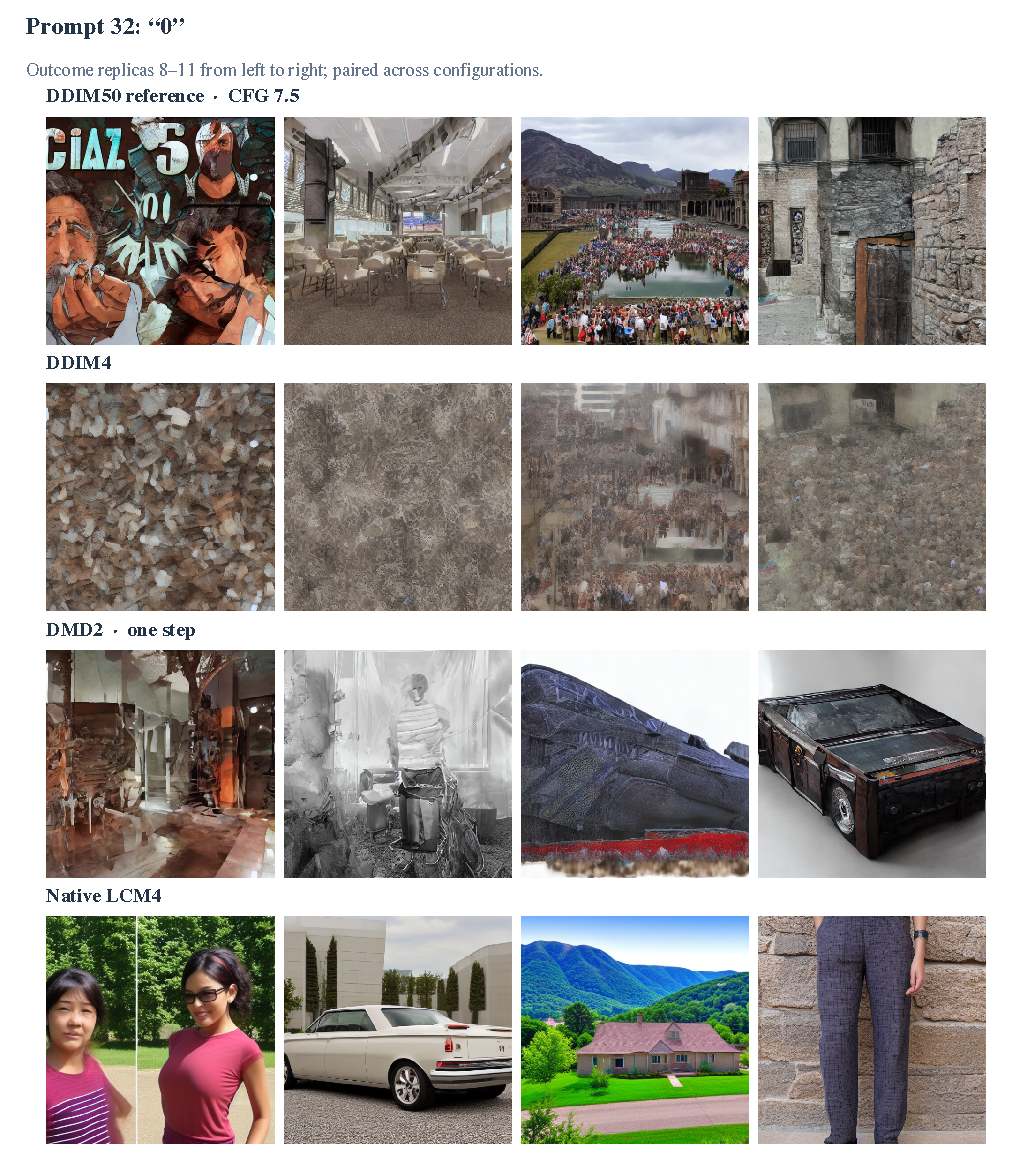
\includegraphics[width=\textwidth]{../figures/t2i_multiseed_0032.pdf}
\caption{Predetermined multi-seed comparison for prompt 32 (``0'').
The three displayed prompts are the smallest held-out original prompt IDs;
columns are outcome replicas 8--11, paired across configurations. The index
rule was recorded before opening images for this display. Every image is
retained without ranking, replacement, or cropping. These abstract prompts
illustrate variation and do not establish semantic coverage.}
\label{fig:t2i_multiseed_32}
\end{figure*}

\begin{figure*}[tp]
\centering
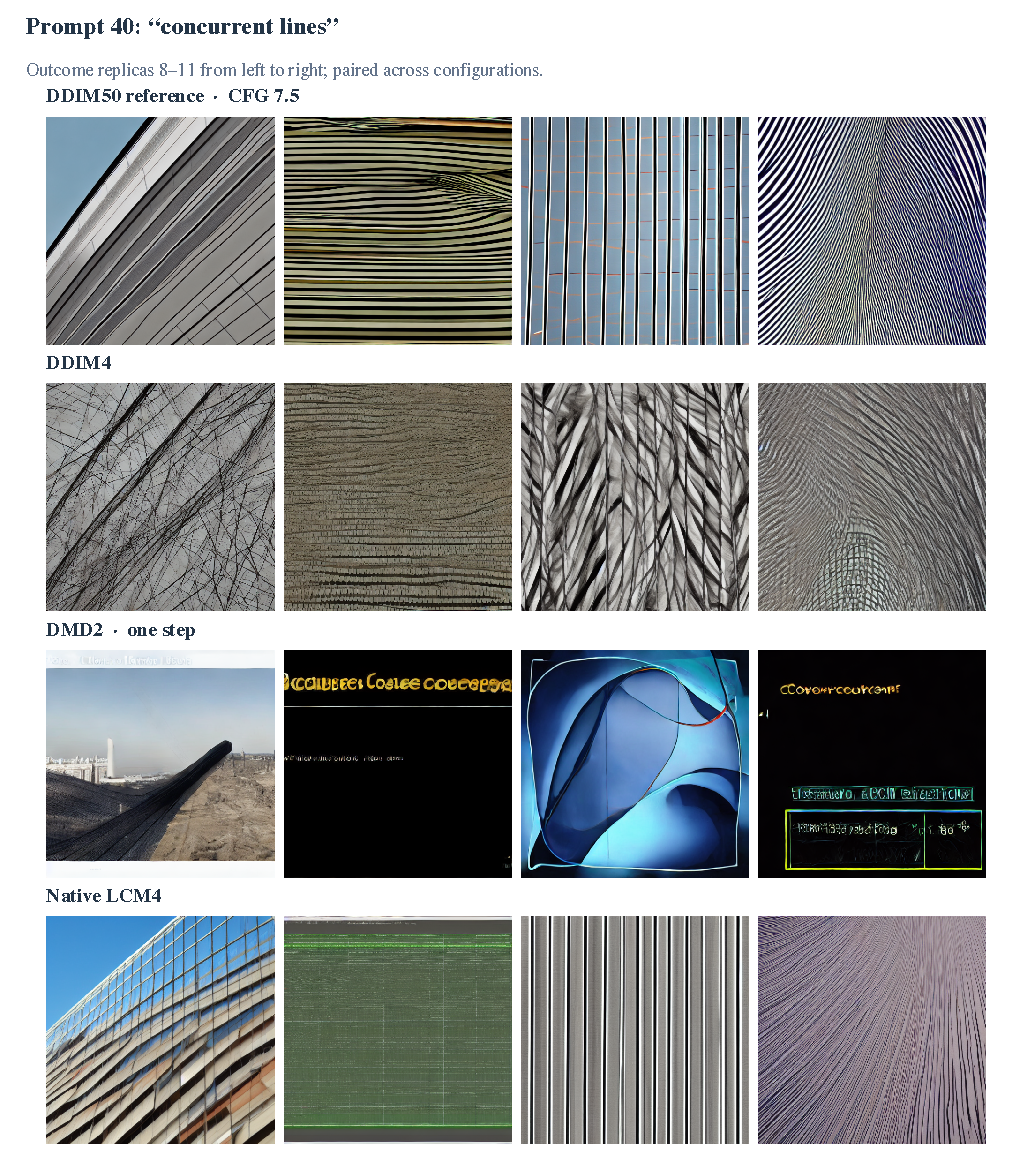
\includegraphics[width=\textwidth]{../figures/t2i_multiseed_0040.pdf}
\caption{Predetermined multi-seed comparison for prompt 40 (``concurrent lines'').
The three displayed prompts are the smallest held-out original prompt IDs;
columns are outcome replicas 8--11, paired across configurations. The index
rule was recorded before opening images for this display. Every image is
retained without ranking, replacement, or cropping. These abstract prompts
illustrate variation and do not establish semantic coverage.}
\label{fig:t2i_multiseed_40}
\end{figure*}

\begin{figure*}[tp]
\centering
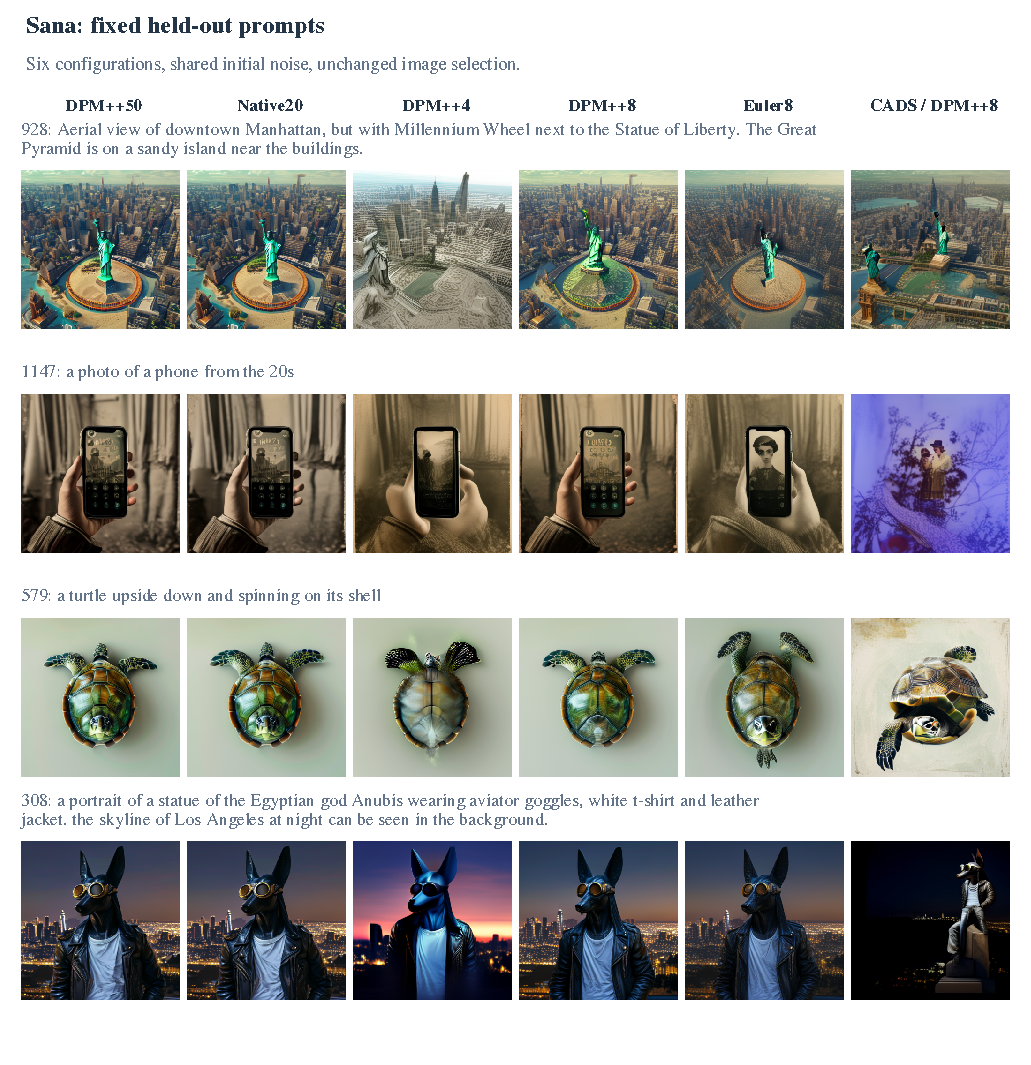
\includegraphics[width=\textwidth]{../figures/t2i_flow_qualitative.pdf}
\caption{Predetermined Sana comparison. Rows are the first four prompts in the
frozen shuffled evaluation order, using outcome replica 8. Columns share
initial noise. The 50-step reference and native20 setting are retained;
all seven configurations, including Euler4, remain in the numerical tables.
Images are neither ranked nor replaced.}
\label{fig:flow_qualitative}
\end{figure*}
